\chapter{Approximations}
\graphicspath{{../gfx/chapter02/}{../plots/chapter02/}}

% TODO: in chapter 1: change V_2 -> V_0
% TODO: chapter one, decomposed Hamiltonian: - H^c_k -> + H^c_k
% TODO: consistent \emph{fixed charge} terminology

\section{Fixed charge model}

Exact diagonalization scales exponentially with system size. For the full
\emph{grand canonical} QCA Hamiltonian, Eq.~\ref{eq:H_QCA}, only QCA devices of
up to two cells are computationally feasible. Therefore, to access larger
systems we need to introduce approximations. Approximating means to simplify.
However, by carefully establishing successive approximations and their limits,
we also reduce the problem to its essential ingredients and thus, hopefully, we
gain a better understanding of the system. As a first step, we reduce the
Hilbert space to a \emph{fixed} number of particles per cell. We disallow any
charge fluctuations, both for the system as a whole and for each individual
cell. With that, we omit the chemical potential term in the Hamiltonian, $\mu =
0$, and prohibit inter-cell hopping. This is a major simplification. However, it
is in line with the QCA idea: The approach requires a fixed number of charges
per cell, typically two electrons, and cells are thought to interact only via
Coulomb forces. In a sense we are shifting the starting point of our
investigation. If the \emph{fixed} charge approximation is not valid for a given
system, then there is no hope of implementing QCA on it. On the other hand, for
experimental systems like the atomic silicon quantum dots and for a given cell
layout, it should always be possible, at least in principle, to tune the system
parameters, especially the chemical potential, to get the system into the right
particle number sector. The system has to be set up in a way that the
two-electrons-per-cell sector is lowest in energy and other particle number
sectors are sufficiently gapped out, that is, at an energy, compared to the
ground state energy, much larger than temperature. Of course, in practice there
are very clear limits as to how much the system parameters can be tuned and any
QCA cell layout considered within the \emph{fixed} charge approximation cannot
necessarily be readily implemented on a given real-world material system.

For the \emph{fixed} charge system, the state space scales as $N_s =
\binom{8}{2}^{N_c} = 28^{N_c}$ ($N_c$ is the number of cells). Using symmetries,
the largest block of the Hamiltonian matrix is the spin zero sector, of size
$N_s^{\prime} = 16^{N_c}$. On conventional computer hardware, systems of up to
four cells are possible, with memory requirements of 32GB. In practice,
however, calculations for four-cell systems take too long and thus three
cells is the practical limit for the \emph{fixed}-number-of-particles-per-cell
model.


\section{Bond model}

%
\begin{figure}
  \center
  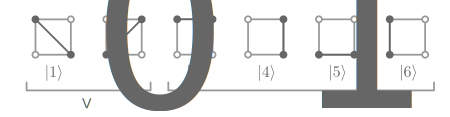
\includegraphics{bond}
  \caption{\ldots}
  \label{fig:bond}
\end{figure}
%
At its heart, QCA is a semi-classical idea. It relies solely on charge-charge
interactions and ignores the particle spins. Therefore, as a next step in our
quest to access larger system sizes, we neglect the spin degree of freedom in
our model. The 28 states per cell of the \emph{fixed} charge model can be
reorganized into four doubly occupied dots and six bonds. The six bonds are
illustrated in Fig.~\ref{fig:bond}. Each bond corresponds to one spin singlet
and three spin triplet states. The \emph{bond} approximation only keeps one
state for each bond and discards the doubly occupied states as well. With the
\emph{bond} model we thus assume that singlet and triplet states are
qualitatively equivalent and energetically degenerate, and that doubly occupied
dots are sufficiently gapped out, that is, $U \gg T$. As QCA ignores the spin,
singlets and triplets should be qualitatively equivalent, but they are not quite
degenerate. We expect that virtual double-occupancy lowers the energies of the
singlet states and therefore introduces a small singlet-triplet splitting.
Still, degeneracy is presumably not a bad assumption to start with and we will
look at the singlet-triplet splitting in detail in due course. For the
\emph{bond} model the QCA Hamiltonian reduces to
%
\begin{equation}
  \label{eq:H_bond}
  H = - \sum_{\left<ij\right>} t c_i^{\dagger} c_j
      + \sum_{i<j} V_{ij} \left( n_i - q \right) \left( n_j - q \right) \, .
\end{equation}
%
With six bond states per cell, the Hilbert space of the \emph{bond} model is
$N_s = 6^{N_c}$ ($N_c$ the number of cells). Five and six cells are doable, with
memory requirements of 460MB and 16GB, respectively, but for practical
calculations five cells really is the limit. For the \emph{bond} model there are
no symmetries that can be exploited.


\section{Ising model}

\newcommand{\ket}[1]{\left|#1\right>}
\newcommand{\bra}[1]{\left<#1\right|}

%
\begin{figure}
  \center
  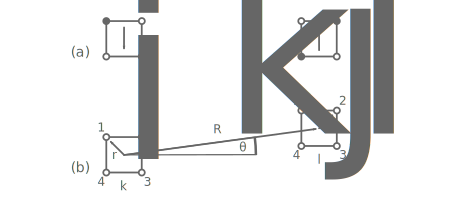
\includegraphics{ising}
  \caption{a) QCA cells $k$ and $l$. b) The two-states-per-cell approximation
  identifies each cell with a spin $\uparrow$ or $\downarrow$.}
  \label{fig:cells2}
\end{figure}
%
A linear array of QCA cells where each cell has a state of logic 0 or 1 is
reminiscent of a 1D spin $\frac{1}{2}$ chain. Indeed, if we reduce the basis to
only two states per cell, down from six states in the \emph{bond} picture, we
can map the QCA system to a transverse-field Ising model with long-ranging
interactions. This is an attractive proposition: The smaller Hilbert space
allows for larger system sizes with our exact diagonalization method; more
importantly, the transverse-field Ising model is amenable to sign-problem-free
Stochastic series expansion (SSE) quantum Monte Carlo schemes
\cite{Sandvik2003}. These methods do not scale exponentially\footnote{SSE
quantum Monte Carlo methods roughly scale as $N \ln N$ where $N$ is the system
size.} and consequently allow access to much larger systems. Last, but not
least, such a mapping connects the QCA approach to the established and well
studied Ising model. The prospect hinges on the assumption that the
two-states-per-cell basis actually is a good approximation for QCA systems. And
while bistable two-state cells are certainly the picture we have in mind when we
talk about QCA, it is not \emph{a priori} clear whether this is a correct
physical picture. 

We use the \emph{bond} Hamiltonian \eqref{eq:H_bond} as the starting point. We
had already discussed in the last chapter that such a Hamiltonian can be
decomposed into single-cell terms and cell-cell interaction terms,
\begin{equation}
  H = \sum_k H^c_k + \sum_{k<l} H^{cc}_{kl} \, .
\end{equation}
In comparison, the transverse field Ising model is described by
%
\begin{equation}
  \tilde{H} = - \sum_k \gamma S^x_k + \sum_{k<l} J_{kl} S^z_k S^z_l \, .
\end{equation}
%
Thus, we would like to map the single cell term $H^c_k$ to the transverse field
term $-\gamma S^x_k$ and the Coulombic cell-cell interaction $H^{cc}_{kl}$ to 
the Ising term $J_{kl} S^z_k S^z_l$. Each cell $k$ is identified with a pseudo
spin $S^z_k$, specifically the logic 0 with a spin down state and the logic 1
with a spin up state, as illustrated in Fig.~\ref{fig:cells2}(b). We will first
look at how the QCA cell can be represented by only two states and derive an
approximate expression for the transverse field $\gamma$. Then we will use a
multipole expansion to derive $J_{kl}$ from the cell-cell Coulomb interaction.
% TODO: maybe point out again that J_{kl} is long-ranged

To arrive at a single-cell-basis with only two states we can, in principle,
follow a similar prescription as for the fixed charge and bond approximations:
We neglect high energy states which are assumed to be gapped out. In this case
these are the four edge states with Coulomb energy $V_1$, $\ket{\psi_Q} =
\left\{ \ket{3}, \ket{4}, \ket{5}, \ket{6} \right\}$ in Fig.~\ref{fig:bond},
where we have introduced $\ket{\psi_Q}$ to denote the high-energy subspace of
the single-cell Hilbert space. We only keep the low-energy, diagonal states
$\ket{\psi_P} = \left\{ \ket{1}, \ket{2} \right\}$ with Coulomb energy $V_0$. Of
course, these two are exactly our logic 0 and logic 1 state, or $\ket{1} \doteq
\ket{\downarrow}$ and $\ket{2} \doteq \ket{uparrow}$, respectively.  Here,
$\ket{\psi_P}$ denotes the low-energy subspace. For the high-energy states to be
sufficiently gapped out we require $\Delta V = V_1 - V_0 \gg T$. In contrast to
the fixed charge and bond models, merely truncating the Hilbert space is not
sufficient for the Ising model. For our previous two approximations the
Hamiltonian had remained essentially unchanged, apart from dropping no longer
relevant terms, such as the chemical potential term or the Hubbard $U$ term. The
retained states were exactly the same states as in the full, untruncated model.
But with only two states per cell the existing Hamiltonian \eqref{eq:H_bond}
does not ``work'': There is no process that takes the system from state
$\ket{1}$ to $\ket{2}$. Therefore, for the Ising approximation we need to derive
an effective, low-energy Hamiltonian from the bond model. In the bond picture,
for the system to transition from state $\ket{1}$ to $\ket{2}$ it can take
different paths, for example $\ket{1} \rightarrow \ket{3} \rightarrow{2}$,
consisting of two hopping processes with an interim high-energy edge state. We
will treat those processes perturbatively, as \emph{virtual} excitations, and
derive an effective hopping term between the two states $\ket{1}$ and $\ket{2}$.
This effective hopping term is precisely the transverse field $\gamma$ which
flips the spin in the Ising picture, $-\gamma S^x_k = -\gamma \frac{1}{2} \left(
S^+_k + S^-_k \right)$.

A single QCA cell is described by the time-independent Schr\"odinger equation
$H^c_k \ket{\psi} = E_k \ket{\psi}$, with $\ket{\psi} = \left[ \ket{\psi_P}
\ket{\psi_Q} \right]$. Our aim it to truncate the basis to $\ket{\psi_P}$ and
derive and an effective Hamiltonian $\tilde{H}^c_k$ with the subspace
Schr\"odinger equation $\tilde{H}^c_k \ket{\psi_p} = E_k \ket{\psi_p}$. The
high-energy states $\ket{\psi_Q}$ have to be incorporated as virtual
excitations.  Using the basis depicted in Fig.~\ref{fig:bond} the single-cell
bond Hamiltonian is very simple and can be written down explicitly. As the
single-cell Hamiltonian is the same for all cells, we can drop the index $k$.
%
\begin{equation}
\begin{split}
  \label{eq:H_marix}
  H^c
  &=
  %
  \left(
  \begin{array}{cc|cccc}
    V_0 & 0   & -t  & -t  & -t  & -t  \\
    0   & V_0 & -t  & -t  & -t  & -t  \\
    \hline
    -t  & -t  & V_1 & 0   & 0   & 0   \\
    -t  & -t  & 0   & V_1 & 0   & 0   \\
    -t  & -t  & 0   & 0   & V_1 & 0   \\
    -t  & -t  & 0   & 0   & 0   & V_1 \\
  \end{array}
  \right) \\[1em]
  %
  &=
  \left(
  \begin{array}{cc}
    H_{PP} & H_{PQ} \\
    H_{QP} & H_{QQ} \\
  \end{array}
  \right)
\end{split}
\end{equation}
%
Here, we have partitioned the Hamiltonian into four blocks, $H_{PP}$, $H_{QQ}$,
$H_{PQ}$, and $H_{QP}$, corresponding to the low-energy subspace $\ket{\psi_P}$,
the high-energy subspace $\ket{\psi_Q}$, and transitioning between the subspaces.
With a this partitioned Hamiltonian the time-independent Schr\"odinger equation
is
%
\begin{equation}
  \label{eq:SE}
  %
  \begin{pmatrix}
    H_{PP} & H_{PQ} \\
    H_{QP} & H_{QQ} \\
  \end{pmatrix}
  \begin{pmatrix}
    \psi_P \\
    \psi_Q \\
  \end{pmatrix}
  =
  E
  \begin{pmatrix}
    \psi_P \\
    \psi_Q \\
  \end{pmatrix}
  %
\end{equation}
%
Writing out the matrix equation as two equations explicitly and eliminating
$\ket{\psi_Q}$ yields 
%
\begin{equation}
  H_{PP} \ket{\psi_P} + H_{PQ} \frac{1}{E - H_{QQ}} H_{QP} \ket{\psi_P}
  =
  E \ket{\psi_P}
\end{equation}
%
and therefore
%
\begin{equation}
  \label{eq:H_effective}
  \tilde{H}^c = H_{PP} + H_{PQ} \frac{1}{E - H_{QQ}} H_{QP} \, .
\end{equation}
%
Assuming that the system is predominantly in the subspace spanned by
$\ket{\psi_P}$ and additionally that the hopping is very small, $t \ll V_0$, we
can approximate $E \approx V_0$. We write out the matrix multiplications and use
$H_{PP} = \left( V_0 \right)_{ii} \delta_{ij}$, $H_{PQ} = \left( -t
\right)_{ij}$, and so on. The effective Hamiltonian becomes
%
\begin{equation}
\begin{split}
  \tilde{H}^c_{ij}
  %
  &=
  \left( V_0 \right)_{ii} \delta_{ij}
  + \left( - t \right)_{ik}
    \left( V_0 - V_1 \right)^{-1}_{kk}
    \left( - t \right)_{kj} \\
  %
  &=
  \left( V_0 \right)_{ii} \delta_{ij}
  - \left( \frac{4 t^2}{\Delta V} \right)_{ij} \, .
\end{split}
\end{equation}
%
As the system remains unchanged upon adding a constant term to the Hamiltonian,
we can subtract the constant diagonal term $\tilde{H}_{ii} = V_0 - \frac{4
t^2}{\Delta V}$, and arrive at
%
\begin{equation}
  \tilde{H}^c
  =
  \begin{pmatrix}
    0 & - \frac{4 t^2}{\Delta V} \\
    - \frac{4 t^2}{\Delta V} & 0 \\
  \end{pmatrix} \, .
\end{equation}
%
The off-diagonal matrix elements are the effective hopping, transitioning the
system between its two states $\ket{1} \leftrightarrow \ket{2}$. If we now
compare this matrix with the transverse field term of the Ising model, where we
use the basis $\ket{\downarrow} \doteq \ket{1}$ and $\ket{\uparrow} \doteq
\ket{2}$, 
%
\begin{equation}
\begin{split}
  \tilde{H}^c
  &=
  - \gamma S^x_k \\
  &=
  - \frac{1}{2} \gamma \left( S^+_k + S^-_k \right) \\[0.5em]
  &= 
  \begin{pmatrix}
    0 & - \frac{1}{2} \gamma \\
    - \frac{1}{2} \gamma & 0 \\
  \end{pmatrix} \, ,
\end{split}
\end{equation}
%
we identify the effective hopping as the transverse field $\gamma$
%
\begin{equation}
  \gamma = \frac{8 t^2}{\Delta V} \, .
\end{equation}
%
The effective hopping $\gamma$ is a virtual process, involving two hopping
processes in the original bond model, yielding the $t^2$ in the numerator of the
expression for $\gamma$, and an interim high-energy state gapped out by $\Delta
V$, hence the $\Delta V$ in the denominator. To arrive at the expression for the
effective hopping we used the assumptions $\Delta V \gg T$ and $t \ll \Delta V$.
As a reminder, $\Delta V = V_1 - V_0 = \frac{2 - \sqrt{2}}{2} \frac{1}{a}
\approx 0.3 V_1$. Notably, the energy gap is independent of the compensation
charge $q$. As the derivation used only a single cell, it is also implicitely
assumed that the perturbations from other cells in the system are small, at
least as far as the effective hopping is concerned. If the hopping depended on
nearby cells' state, then the effective Hamiltonian would be much more involved
and certainly could not be mapped to an Ising-like model.

We have successfully derived an effective hopping term and therefore also an
effective two-state model for the QCA Hamiltonian. With only two states per cell
the Hilbert space scales as $N_s = 2^{N_c}$ ($N_c$ the number of cells) and up
to 14 cells are computationally feasible, with memory requirements of 2GB. In
practice we restrict the calculations to a maximum of 12 or 13 cells. For our
calculations we can use the two-state approximation with the effective hopping
term, but still retain the original cell-cell interaction term $H^{cc}_{kl}$.
Summing up all cell-cell interactions exactly is no problem for the relatively
small system sizes accessible with exact diagonalization.  Thus, from a
computational point of view, nothing is gained by expressing the cell-cell
interaction as an Ising interaction. However, deriving $J_{kl}$ from
$H^{cc}_{kl}$ is very rewarding conceptually and enables us to properly map the
QCA approach to an Ising model. Additionally, an analytical expression for
$J_{kl}$ will already allow some key insights into the characteristics of QCA
devices. Therefore, we now undertake the derivation of an approximate expression
for $J_{kl}$ via a multipole expansion. The obvious starting point is the
cell-cell interaction term $H^{cc}_{kl}$, 
%
\begin{equation}
\begin{split}
  H^{cc}_{kl} 
  %
  &=
  %
  \sum_{\substack{i \in k\\j \in l}} V_{ij} \left( n_i - q \right) \left( n_j - q \right) \\
  %
  H^{cc}_{kl}
  %
  &= 
  %
  \sum_{\substack{i \in k\\j \in l}}
  \frac{ \left( n_i - q \right) \left( n_j - q \right) }
       { \left| \bm{R}_{kl} + \bm{r}_j - \bm{r}_i \right| } \\
  %
  &=
  \sum_{\substack{i \in k\\j \in l}}
  \frac{n_i n_j - q (n_i + n_j)}
       {\left| \bm{R}_{kl} + \bm{r}_{ij} \right|} \, ,
\end{split}
\end{equation}
%
where $i$ and $j$ sum over the four dots $1\ldots4$ of cell $k$ and $l$,
respectively, $\bm{R}_{kl}$ denotes the vector between the centres of the cells,
see Fig.~\ref{fig:cells2}(a). We have introduces $\bm{r}_{ij} = \bm{r}_j -
\bm{r}_i$ and dropped the constant $q^2$ term. There are only four possible
configurations for two interacting cells, $\uparrow\uparrow$,
$\downarrow\downarrow$, $\uparrow\downarrow$, and $\downarrow\uparrow$, and we can
calculate their energies explicitely. For example, with the shorthand notations
$V_{ij} = \frac{1}{\left| \bm{R}_{kl} + r_{ij} \right|} + \frac{1}{\left|
\bm{R}_{kl} - r_{ij} \right|}$ and $V_{00} = \frac{1}{\left| \bm{R}_{kl}
\right|}$, the Coulomb energy for two spin-up cells is written
\begin{equation}
  \label{eq:E_upup}
  %
  E^{\uparrow\uparrow}
  =
  2 \left( 1 - 2 q \right) \left[ V_{00} + V_{24} \right]
  - 2 q \left[ V_{12} + V_{14} \right] \, .
\end{equation}
The energy for two spin-down cells can be obtained simply by rotating the system
by $90^{\circ}$ and thus by permutating the dot numbering in the expression
above, $2,3,4,1 \rightarrow 1,2,3,4$. Using symmetries, for example $V_{43} =
V_{12}$, we arrive at
\begin{equation}
  \label{eq:E_downdown}
  %
  E^{\downarrow\downarrow}
  =
  2 \left( 1 - 2 q \right) \left[ V_{00} + V_{13} \right]
  - 2 q \left[ V_{12} + V_{14} \right] \, .
\end{equation}
The remaining two configurations' energies can be calculated similarly and we
find $E^{\uparrow\downarrow} = E^{\downarrow\uparrow}$, which, given the highly
symmetric geometry of the cell arrangement, does not come as a suprise. But
crucially, in general we have $E^{\uparrow\uparrow} \ne
E^{\downarrow\downarrow}$. Therefore we have a system with three distinct energy
levels which we cannot hope to represent with the solely two-level Ising term
$J_{kl} S^z_l S^z_l$. Instead, let us try to map to a \emph{modified} Ising model
with a three-level cell-cell interaction term of the form
%
\begin{equation}
  \tilde{H}^{cc}_{kl}
  = 
  J_{kl} S^z_k S^z_l + 
  J^{\prime}_{kl} \left( S^z_k + S^z_l \right) \, .
\end{equation}
%
For this Hamiltonian we have the energies
%
\begin{align}
  \tilde{E}^{\uparrow\uparrow} - \tilde{E}^{\uparrow\downarrow}
  &=
  2J_{kl} + 2J^{\prime}_{kl} \\
  %
  \tilde{E}^{\downarrow\downarrow} - \tilde{E}^{\uparrow\downarrow}
  &=
  2J_{kl} - 2J^{\prime}_{kl}
\end{align}
%
which yields
%
\begin{align}
  \label{eq:Js_from_Es}
  J_{kl}
  &=
  \frac{1}{4} 
  \left( 
    \tilde{E}^{\uparrow\uparrow} + \tilde{E}^{\downarrow\downarrow}
    - 2 \tilde{E}^{\uparrow\downarrow} 
  \right) \\
  %
  J^{\prime}_{kl}
  &=
  \frac{1}{4}
  \left( \tilde{E}^{\uparrow\uparrow} - \tilde{E}^{\downarrow\downarrow} \right) \, .
\end{align}
%
To map the bond cell-cell interaction $H^{cc}_{kl}$ to the modified Ising
interaction term we identify $E^{\uparrow\uparrow} =
\tilde{E}^{\uparrow\uparrow}, E^{\downarrow\downarrow} =
\tilde{E}^{\downarrow\downarrow}$, and so on. The newly introduced
$J^{\prime}_{kl}$ term tracks the difference between $E^{\uparrow\uparrow}$ and
$E^{\downarrow\downarrow}$. Going back to the expressions \eqref{eq:E_upup} and
\eqref{eq:E_downdown} we realize that for $q = \frac{1}{2}$---charge neutral
cells---they \emph{do} become equal, $E^{\uparrow\uparrow} =
E^{\downarrow\downarrow}$, and therefore $J^{\prime}_{kl} = 0$. This is an
important result: Only for charge neutral cells does the QCA model map to a
genuine, unmodified transverse field Ising model.

To obtain concrete expressions for $J_{kl}$ and $J^{\prime}_{kl}$ we do a
multipole expansion of $E^{\uparrow\uparrow}, E^{\downarrow\downarrow},
E^{\uparrow\downarrow}$, and $E^{\downarrow\uparrow}$. Specifically,
%
\begin{equation}
\begin{split}
  \frac{1}{\left| \bm{R}_{kl} \pm r_{ij} \right|}
  &=
  \frac{1}{R}
  \left( 
    1 \pm 2 \frac{\bm{r}_{ij} \hat{\bm{R}}}{R} + \frac{r_{ij}^2}{R^2}
  \right)^{-1/2} \\
  &=
  \frac{1}{R} \left( 1 \pm x + y \right)^{-1/2}
\end{split}
\end{equation}
%
is Taylor-expanded in $x$ and $y$, keeping all terms up to
$\mathcal{O}\left(\frac{a^4}{R^5}\right)$ which corresponds to
quadrupole-quadrupole interactions. Plugging the multipole-expanded energies
into Eq.~\eqref{eq:Js_from_Es} yields the final expressions
%
\begin{align}
  %
  J_{kl}
  &=
  \frac{ 1 }{ 32 }
  \left(
    9 - 105 \cos{4 \theta}
  \right)
  \frac{ a^4 }{ R_{kl}^5 }
  \\
  %
  J^{\prime}_{kl}
  &=
  \left( 1 - 2 q \right)
  \left(
    \frac{ 3 }{ 2 } \sin{2 \theta} \frac{ a^2 }{ R_{kl}^3 } +
    \frac{ 5 }{ 4 } \sin{2 \theta} \frac{ a^4 }{ R_{kl}^5 }
  \right) \, .
  %
\end{align}
%
We have successfully mapped the QCA bond Hamiltonian \eqref{eq:H_bond} to a
modified transverse field Ising model
\begin{equation}
  \label{eq:H_Ising}
  %
  \tilde{H}
  =
  - \sum_k \gamma S^x_k
  + \sum_{k<l}
    \left[
      J_{kl} S^z_k S^z_l + 
      J^{\prime}_{kl} \left( S^z_k + S^z_l \right)
    \right] \, ,
\end{equation}
which reduces to a genuine Ising model, $J^{\prime}_{kl} = 0$, in the case of
charge neutral cells, $q = 0$.

These results are remarkable in two ways. First, $J_{kl}$ does not depend on the
compensation charge $q$. In turn, the Ising interaction $J_{kl}
S^z_k S^z_l$ is independent of the cell net charge and represents only
the quadrupole-quadrupole interaction, falling off as $J_{kl} \sim R_{kl}^{-5}$.
Second, the $J^{\prime}_{kl}$ term does depend on the compensation charge but
vanishes for $q = \frac{1}{2}$, that is, charge neutral cells. For charge
neutral cells QCA therefore maps directly to a normal (unmodified) Ising model.

We can also look at the angle dependence of the interactions. The $J_{kl}$ term is
symmetric under rotations by $90^{\circ}$---which is what we expect
intuitively---whereas the $J^{\prime}_{kl}$ is symmetric under rotations by
$180^{\circ}$. Thus, by slowly turning on $J^{\prime}_{kl}$ (by, for example, going
from charge neutral to effectively negatively charged cells $q = \frac{1}{2}
\rightarrow q = 0$), we break the $90^{\circ}$ rotational invariance. It is
important to note that the $J^{\prime}_{kl}$ term also breaks the symmetry between
spin up and spin down cells. For $J^{\prime}_{kl} \ne 0$, $\uparrow\uparrow$ and
$\downarrow\downarrow$ have different energies and therefore also different
polarization responses. For a practical implementation this is definitely not
what we want! At the angles $0^{\circ}, 90^{\circ}$, and $270^{\circ}$
$J^{\prime}_{kl}$ vanishes, so here we have a pure Ising interaction even for $q
\ne 0$. Conversely, $J_{kl}$ also vanishes at select angels, rendering the system
bare any interaction for charge neutral cells, at least within the limits of our
multipole expansion.

% more about multipole, what it means, e.g. exact for large distances; that, in
% principle, the cutoff of the expansion is arbitrary and we can make it exact
% by including higher order terms. 


\section{Validity of the approximations}



%
\begin{figure}
  \center
  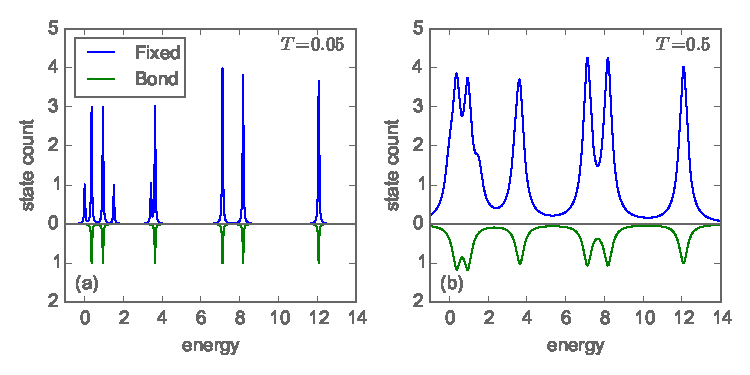
\includegraphics{bond_approximation1}
  \caption{Low-energy density of states of a one cell QCA system for both the
  \emph{fixed charge} and the \emph{bond} model. The \emph{bond} approximation
  does not reproduce the singlet-triplet splitting.}
  \label{fig:bond_approximation1}
\end{figure}
%
\begin{figure}
  \center
  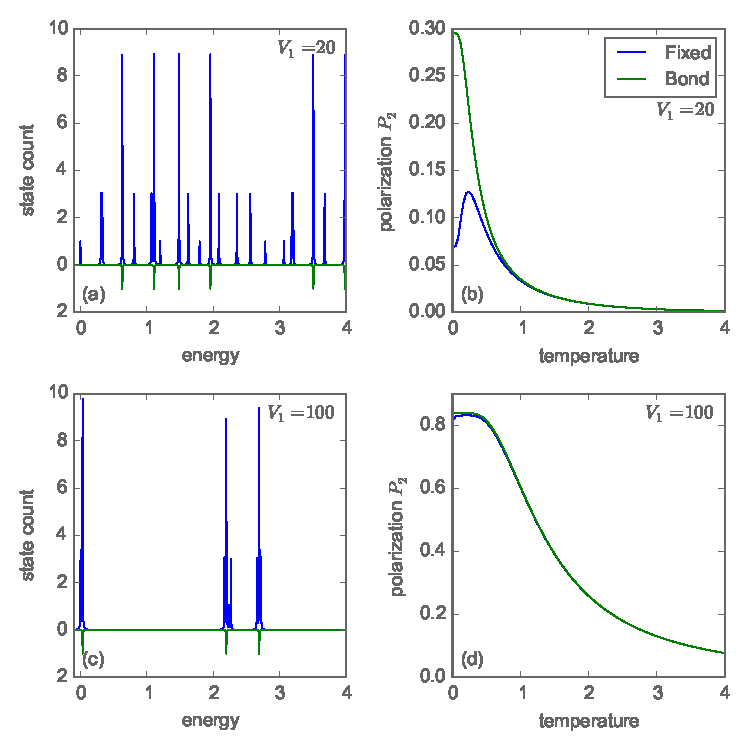
\includegraphics{bond_approximation2}
  \caption{The two cell \emph{fixed charge} and \emph{bond} systems at $V_1 =
  20$ and $V_1 = 100$. (a)(c) Low-energy density of states. (b)(d) Output
  polarization $P_2$ over temperature. For a small Coulomb repulsion the density
  of states curves look qualitatively very different (a) and the \emph{bond}
  approximation does not work very well (b). At a larger Coulomb repulsion the
  density of states curves look much more alike (c) and the \emph{bond}
  approximation works much better (d).}
  \label{fig:bond_approximation2}
\end{figure}
%
%
\begin{figure}
  \center
  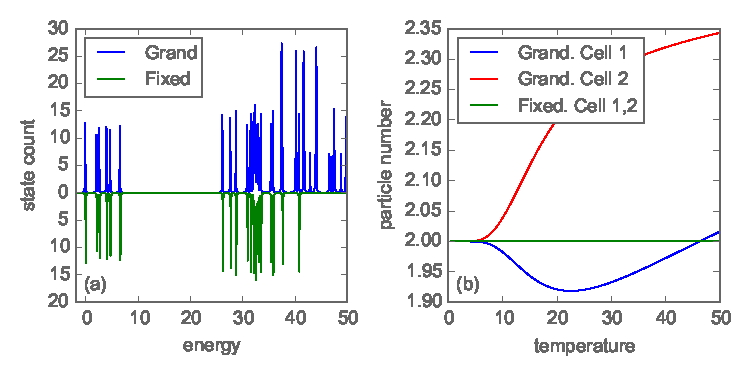
\includegraphics{fixed_charge_approximation}
  \caption{(a) Low-energy density of states of the exact \emph{grand canonical}
  and the approximative \emph{fixed charge} two cell QCA system. For small
  energies the curves agree perfectly (up to $E \lesssim 35$). (b) Particle
  number per cell over temperature for the same two cell system. The curves
  diverge for $T \gtrsim 5$.}
  \label{fig:fixed_charge_approximation}
\end{figure}
%
%
\begin{figure}
  \center
  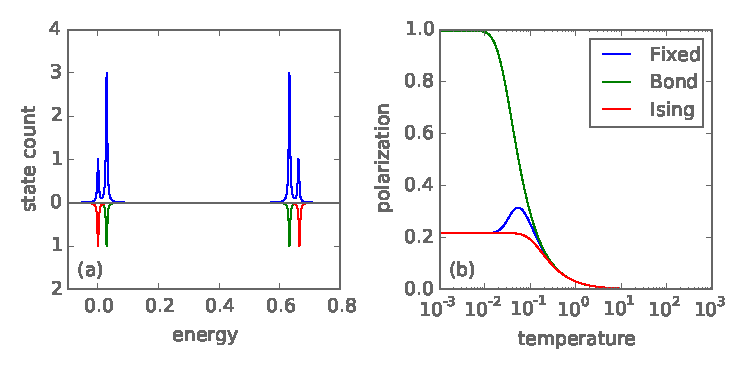
\includegraphics{ising_approximation1}
  \caption{\ldots}
  \label{fig:ising_approximation1}
\end{figure}
%
%
\begin{figure}
  \center
  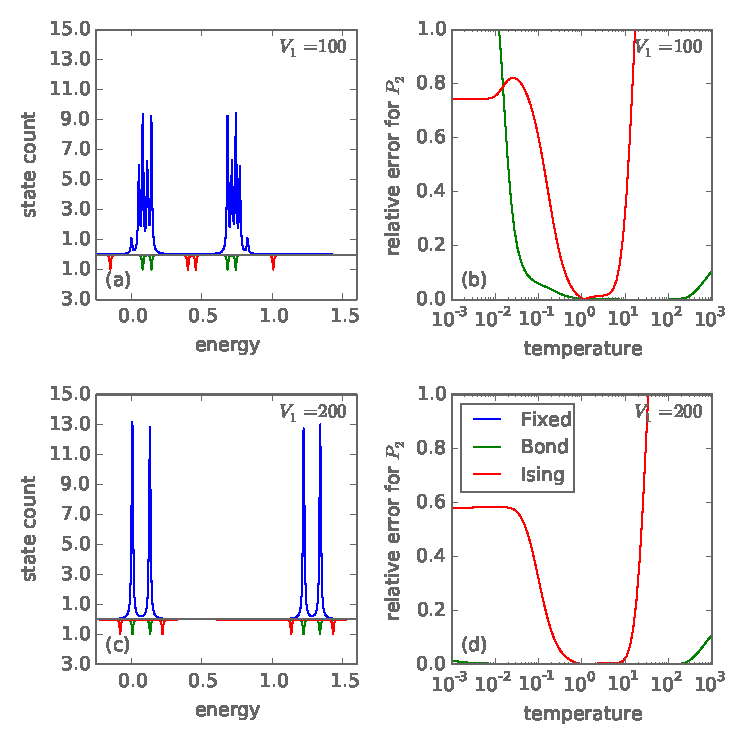
\includegraphics{ising_approximation2}
  \caption{\ldots}
  \label{fig:ising_approximation2}
\end{figure}
%
%
\begin{figure}
  \center
  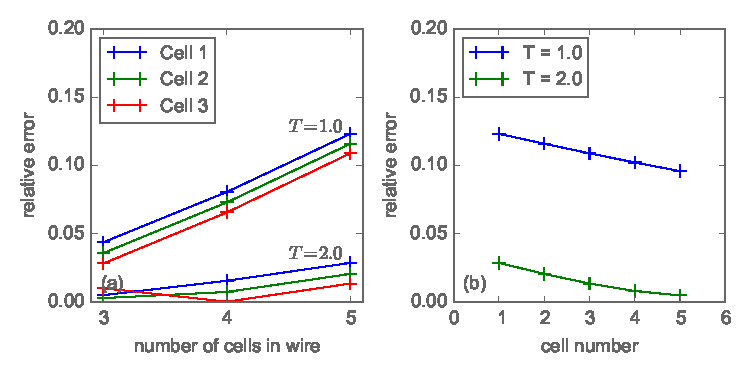
\includegraphics{ising_approximation3}
  \caption{\ldots}
  \label{fig:ising_approximation3}
\end{figure}
%





%%%%%%%%%%%%%%%%%%%%%%%%%%%%%%%%%%%%%%%%%%%%%%%%%%%%%%%%%%%%%%%%%%%%%%%%%%%%%%


% To access larger systems we need to introduce approximations. Approximating
% means to simplify. However, by carefully establishing successive approximations
% and their limits, we also reduce the problem to its essential ingredients and
% thus, hopefully, we gain a better understanding of the system. Our first
% approximation is somewhat ad hoc and motivated by the very ideas underlying the
% QCA approach. QCA relies on two electrons per cell (or, more generally, a fixed
% number of charges per cell). Therefore we truncate the Hilbert space and keep
% only states with two electrons in each cell. We omit the chemical potential
% term, $\mu = 0$. This \emph{fixed charge} approximation obviously does not allow
% for charge fluctuations and consequently cannot accommodate inter-cell hopping.
% We justify the approximation by noting that, at least in principle, for any
% given cell layout we can always tune the system parameters (especially the chemical
% potential) so that we have two electrons per cell. Of course, in practice there
% are very clear limits as to how much system parameters can be tuned and any QCA
% cell layout considered within the \emph{fixed charge} approximation cannot
% necessarily be readily implemented on a given real-world material system.
% 
% For the \emph{fixed charge} system, the state space scales as $N_s =
% \binom{8}{2}^{N_c} = 28^{N_c}$ ($N_c$ is the number of cells). Again, we utilize
% symmetries to make the Hamiltonian matrix block diagonal and as before the
% largest block is the spin zero sector, of size $N_s^{\prime} = 16^{N_c}$. This
% corresponds to a memory consumption of 512kB, 128MB, and 32GB for two, three and
% four cell systems, respectively. That's doable. Five cells, however, remain
% impossible. To illustrate how the approximation works
% Fig.~\ref{fig:fixed_charge_approximation}(a) compares the density of states
% (more correctly, the energy state histogram) of both the \emph{fixed charge}
% and the exact \emph{grand canonical} system. The \emph{fixed charge}
% approximation accurately reproduces the low-energy spectrum of the \emph{grand
% canonical} model. This is not unexpected. As long as the QCA system is in the
% right regime, the two-electrons-per-cell sector is lowest in energy. It is in
% this limit, with the temperature additionally smaller than the energy gap to the
% next higher charge sector, that the approximation is valid.
% Fig.~\ref{fig:fixed_charge_approximation}(b) demonstrates the breakdown of the
% approximation. Here we have plotted the particle number per cell over
% temperature and as the temperature is increased and becomes comparable to the
% energy gap, the \emph{fixed charge} and \emph{grand canonical} systems diverge.
% %
% \begin{figure}
%   \center
%   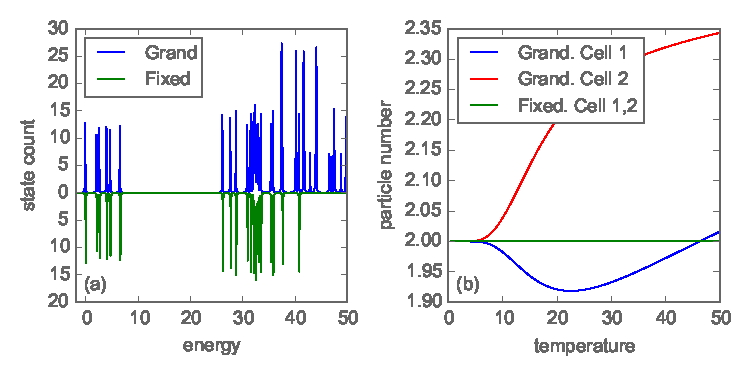
\includegraphics{fixed_charge_approximation}
%   \caption{(a) Low-energy density of states of the exact \emph{grand canonical}
%   and the approximative \emph{fixed charge} two cell QCA system. For small
%   energies the curves agree perfectly (up to $E \lesssim 35$). (b) Particle
%   number per cell over temperature for the same two cell system. The curves
%   diverge for $T \gtrsim 5$.}
%   \label{fig:fixed_charge_approximation}
% \end{figure}
% %




% As evidenced by our semi-classical introduction at the beginning of this report,
% the QCA approach does not consider particle spins. It solely relies on
% charge-charge interactions. Therefore it is natural to the QCA approach to
% neglect the spin degree of freedom as a next step. The 28 states per cell of the
% \emph{fixed charge} model can be reorganized into four doubly occupied dots and
% six bonds, four along the edges and two along the diagonals of the cell. Each
% bond consists of two electrons and corresponds to four states, one spin singlet
% and three spin triplets. By keeping only one state for each bond and omitting
% the doubly occupied states we arrive at the \emph{bond} approximation. It has a
% basis of six states per cell, the six bonds. As a consequence, the size of the
% Hilbert space is $N_s = 6^{N_c}$ ($N_c$ the number of cells). Five and six cells
% are doable, with memory requirements of 460MB and 16GB, respectively, whereas
% seven cells are not (580GB). Note that for the \emph{bond} model there are no
% symmetries that can be exploited. 
% 
% %
% \begin{figure}
%   \center
%   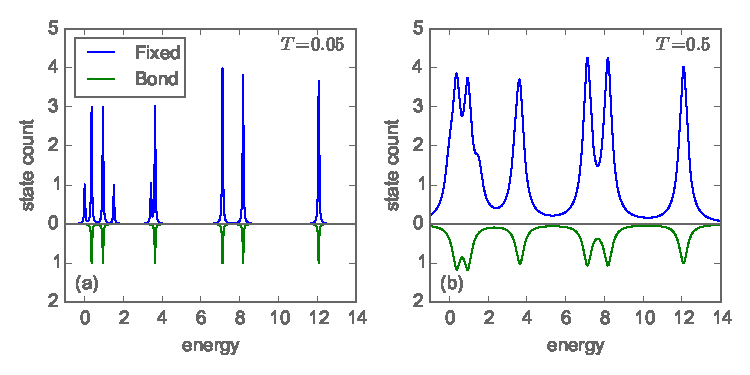
\includegraphics{bond_approximation1}
%   \caption{Low-energy density of states of a one cell QCA system for both the
%   \emph{fixed charge} and the \emph{bond} model. The \emph{bond} approximation
%   does not reproduce the singlet-triplet splitting.}
%   \label{fig:bond_approximation1}
% \end{figure}
% %
% \begin{figure}
%   \center
%   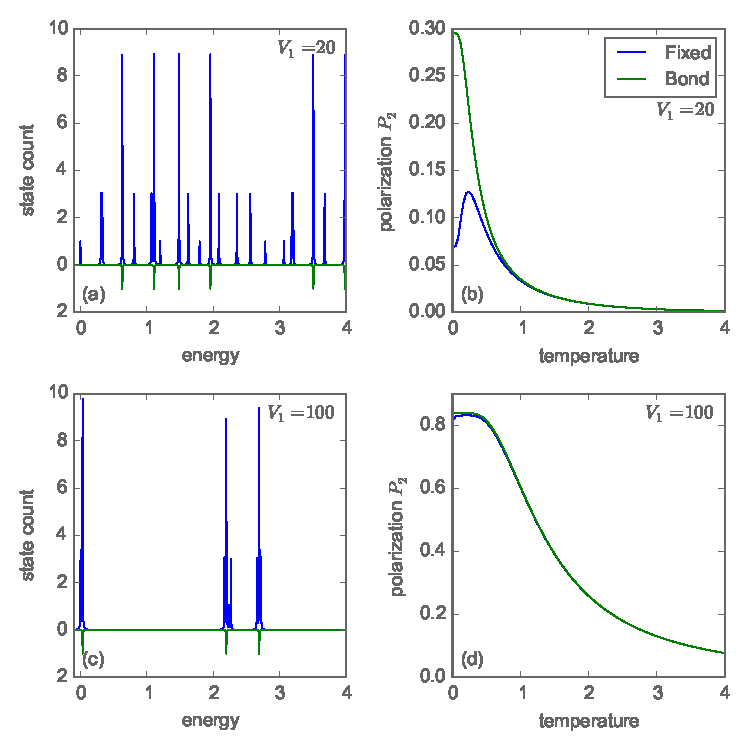
\includegraphics{bond_approximation2}
%   \caption{The two cell \emph{fixed charge} and \emph{bond} systems at $V_1 =
%   20$ and $V_1 = 100$. (a)(c) Low-energy density of states. (b)(d) Output
%   polarization $P_2$ over temperature. For a small Coulomb repulsion the density
%   of states curves look qualitatively very different (a) and the \emph{bond}
%   approximation does not work very well (b). At a larger Coulomb repulsion the
%   density of states curves look much more alike (c) and the \emph{bond}
%   approximation works much better (d).}
%   \label{fig:bond_approximation2}
% \end{figure}
% %
% Apart from requiring sufficiently gapped out doubly occupied states, the
% \emph{bond} approximation assumes that the bond singlet and triplet states are
% energetically degenerate. But this is not quite correct. To understand
% how the approximation works we look at the density of states (energy state
% histogram, to be correct) of the single cell \emph{fixed charge} and \emph{bond}
% systems, Fig.~\ref{fig:bond_approximation1}. Each \emph{bond} state maps to
% three \emph{fixed charge} states---the triplet---and one ``close-by''
% state---the singlet. Hence, singlet and triplet states are not equivalent, they
% are split by an energy gap $\Delta E$. We speculate that, similar to the
% antiferromagnetic Heisenberg coupling constant $J$ emerging in the low energy
% limit of the Hubbard model (with $J \sim \frac{t^2}{U}$) \cite{Auerbach}, here,
% virtual excitations to high energy doubly occupied states lower the energy of
% the singlet state compared to the triplet state. Since the \emph{bond} model
% ignores the singlet-triplet splitting it is important to understand how this gap
% depends on various system parameters. To that end we picked out a few
% selected singlet-triplet states from the spectrum in
% Fig.~\ref{fig:bond_approximation1} as examples. Contrary to expectations, for
% those states the gap $\Delta E$ did not change significantly with the on-site
% Coulomb repulsion $U$, however, it did decrease with decreasing $b$, the
% inter-cell spacing. Most importantly, for the nearest-neighbour Coulomb
% potential, $V_1 = \frac{1}{a}$ ($a$ being the cell side length), we found
% $\Delta E \sim \frac{1}{V_1^p}$. The exponent is $p \sim 3$ when the cell
% ``sees'' a biasing external potential (e.g.\ $P_0 = \pm 1$) and $p \sim 1$
% otherwise (e.g.\ $P_0 = 0$). Even though our method is anything but rigorous and
% the obtained results very likely not universally true, the findings should
% nonetheless give a good enough idea of the principle trends. Quite generally,
% the higher the overall Coulomb potential (large $V_1$, small $b$), the smaller
% the singlet-triplet splitting and, conceivably, the more accurate the
% \emph{bond} approximation.
% 
% We expect the approximation to work as long as the
% singlet-triplet splitting is ``washed out,'' that is, as long as the temperature
% is much bigger than the gap $\Delta E$. As a very, very rough estimate we come
% up with $T \gg \frac{t^2}{V_1}$. Of course, we also need $T \ll U$ so that the
% doubly occupied states are gapped out. Outside of this loosely defined regime,
% the \emph{bond} model can and does go terribly wrong. Especially the ground
% state is often qualitatively completely incorrect. Consider, for example,
% Fig.~\ref{fig:bond_approximation2}(b) where we have plotted the output
% polarization $P_2$ of a two cell system over temperature. For this system we set
% the input polarization $P_0 = 1$, the Hubbard $U$ is practically infinite, the
% inter-cell spacing is $b = 2 a$, and the nearest-neighbour Coulomb repulsion has
% the value $V_1 = \frac{1}{a} = 20$ (in units of $t$, $t=1$). The two curves for
% the \emph{fixed charge} and the \emph{bond} system disagree at low temperatures.
% It is instructive to compare the density of states of the two systems,
% Fig.~\ref{fig:bond_approximation2}(a): They look quite different, qualitatively.
% In that light it is rather remarkable that the polarization curves actually
% agree quite well at higher temperatures ($T > 1$). The \emph{bond} model only
% reproduces the most populous energy states of the exact spectrum. Apparently,
% that is enough to give (almost) correct results at high temperatures. The lower
% the temperature, the more important become the few lowest lying energy states
% which the \emph{bond} model misses. For a larger Coulomb repulsion, $V_1 = 100$,
% the density of states curves look much more alike, even though the \emph{bond}
% model obviously still does not resolve all the lines of the exact spectrum,
% Fig.~\ref{fig:bond_approximation2}(c). Accordingly, the approximation works much
% better as can be seen in Fig.~\ref{fig:bond_approximation2}(d). As a last
% remark, note that for the two cell system each single \emph{bond} state
% corresponds to $16$ ($4 \cdot 4$) \emph{fixed charge} states.




% % 
% \begin{align}
%   J 
%   &=
%   \frac{1}{32}
%   \frac{9 a^4 - 105 a^4 \cos{4\theta}}{R^5} \\
%   %
%   J^{\prime}
%   &=
%   - \frac{1}{4}
%   \left(
%     \frac{6 a^2 \sin{2\theta}}{R^3} + \frac{5 a^4 \sin{2\theta}}{R^5}
%   \right) \, .
% \end{align}
% %
% In the limit $\frac{a}{R} \ll 1$ and together with the (conjectured) kinetic
% single cell term $-\gamma \sigma^x_k$ we have thus mapped the two-state QCA
% system to a transverse-field Ising model, albeit with an additional $J^{\prime}$
% term. The interactions decrease as $\frac{1}{R^3}$ and $\frac{1}{R^5}$ for
% $J^{\prime}$ and $J$, respectively. Both $J$ and $J^{\prime}$ vary with the
% angle $\theta$ between the two cells. As a consequence, different directions
% prefer different cell configurations ($\uparrow\uparrow$ versus
% $\downarrow\downarrow$) and only few select angles yield a pure Ising
% interaction $J_{kl} \sigma^z_k \sigma^z_l$---for example a linear array of cells
% ($\theta = 0^{\circ}$). This is significant as it breaks the symmetry between
% digital 0 and 1 (spin $\downarrow$ and $\uparrow$) for QCA devices if we are not
% very careful in how we engineer them. Moreover, the pure Ising interaction seems
% to be quite fragile with respect to angle displacement, as demonstrated in
% Fig.~\ref{fig:energies}. Here we have plotted the energies $E^{\uparrow\uparrow}
% = J + 2 J^{\prime}$, $E^{\downarrow\downarrow} = J - 2 J^{\prime}$, and
% $E^{\uparrow\downarrow} = E^{\downarrow\uparrow} = - J$.

